% =====================================================================
%  Người A -- Task 2: Mô hình hóa hệ thống
%  Nguồn: docs/diagrams/*.puml, docs/order/state-machine.md,
%         docs/database-design.md, apps/api/prisma/schema.prisma
%  Ngân sách: ~5 trang
% =====================================================================
\section{Task 2 -- Mô hình hóa hệ thống}

% TODO(A): 1 câu dẫn: 3 sơ đồ dùng chung một bộ mã FR/UC với Task 1 và mô hình dữ liệu.
% Mỗi sơ đồ phải có: nguồn .puml/.drawio + ảnh .svg kết xuất (yêu cầu đề).

\subsection{Task 2.1 -- Activity diagram}

% TODO(A): gộp 7 activity trong docs/diagrams/activity-*.puml thành 1 sơ đồ end-to-end
% có 5 swimlane: Khách hàng | Next.js | NestJS API | PostgreSQL | ZaloPay.
% Bắt buộc thể hiện: điểm bắt đầu/kết thúc, decision/merge,
%   - hết nguyên liệu (FR-09),
%   - chưa đăng nhập (FR-04),
%   - thanh toán thất bại + retry (FR-05, FR-08),
%   - huỷ đơn + hoàn kho/điểm (FR-07).
\begin{figure}[H]
\centering
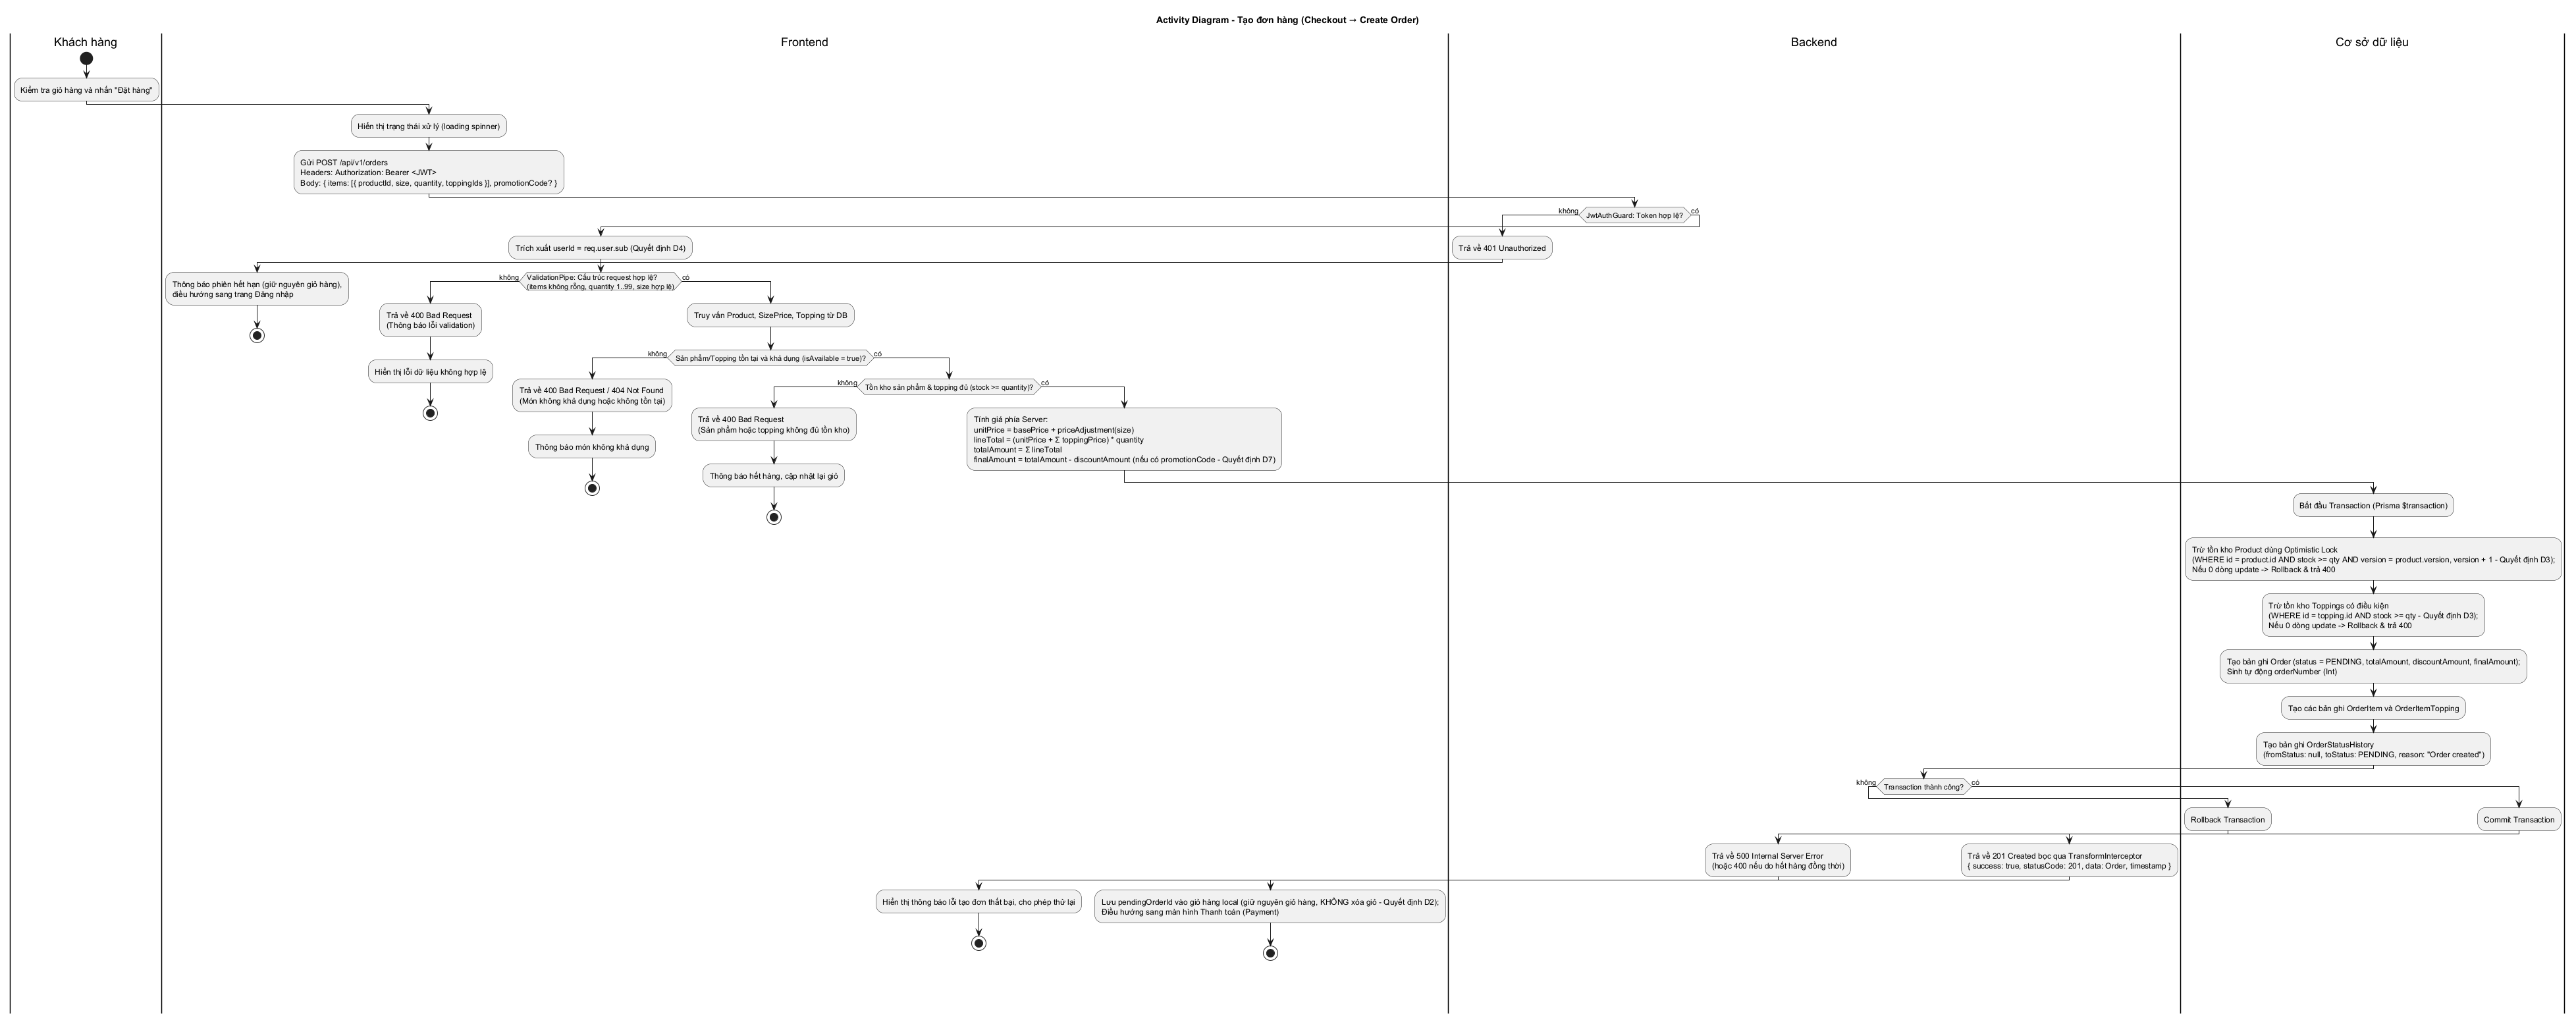
\includegraphics[width=0.92\textwidth]{../figures/diagrams/activity-order.png}
\caption{Activity diagram luồng đặt đơn (bản hiện có -- thay bằng sơ đồ end-to-end có swimlane)}
\label{figA:activity}
\end{figure}

\paragraph{Bảng quyết định.}
% TODO(A): bảng các decision node: mã | điều kiện | nhánh đúng | nhánh sai | FR.
\begin{table}[H]
\centering\small
\caption{Các điểm rẽ nhánh trong activity diagram}
\label{tabA:activity-decision}
\begin{tabularx}{\textwidth}{@{}c X X X@{}}
\toprule
\textbf{Mã} & \textbf{Điều kiện} & \textbf{Nhánh thành công} & \textbf{Nhánh thất bại} \\
\midrule
% TODO(A)
\bottomrule
\end{tabularx}
\end{table}

\subsection{Task 2.2 -- Sequence diagram}

% TODO(A): 5 lifeline bắt buộc: Customer -> Next.js UI -> NestJS API -> Database -> Payment Service.
% Phải thể hiện: request/response, kiểm tra JWT + validate DTO, transaction tạo đơn + cập nhật kho,
% alt thanh toán thành công/thất bại, idempotency khi client gửi lại, thông báo kết quả cuối.
% Nguồn: docs/diagrams/sequence-checkout.puml (đã có).
\begin{figure}[H]
\centering
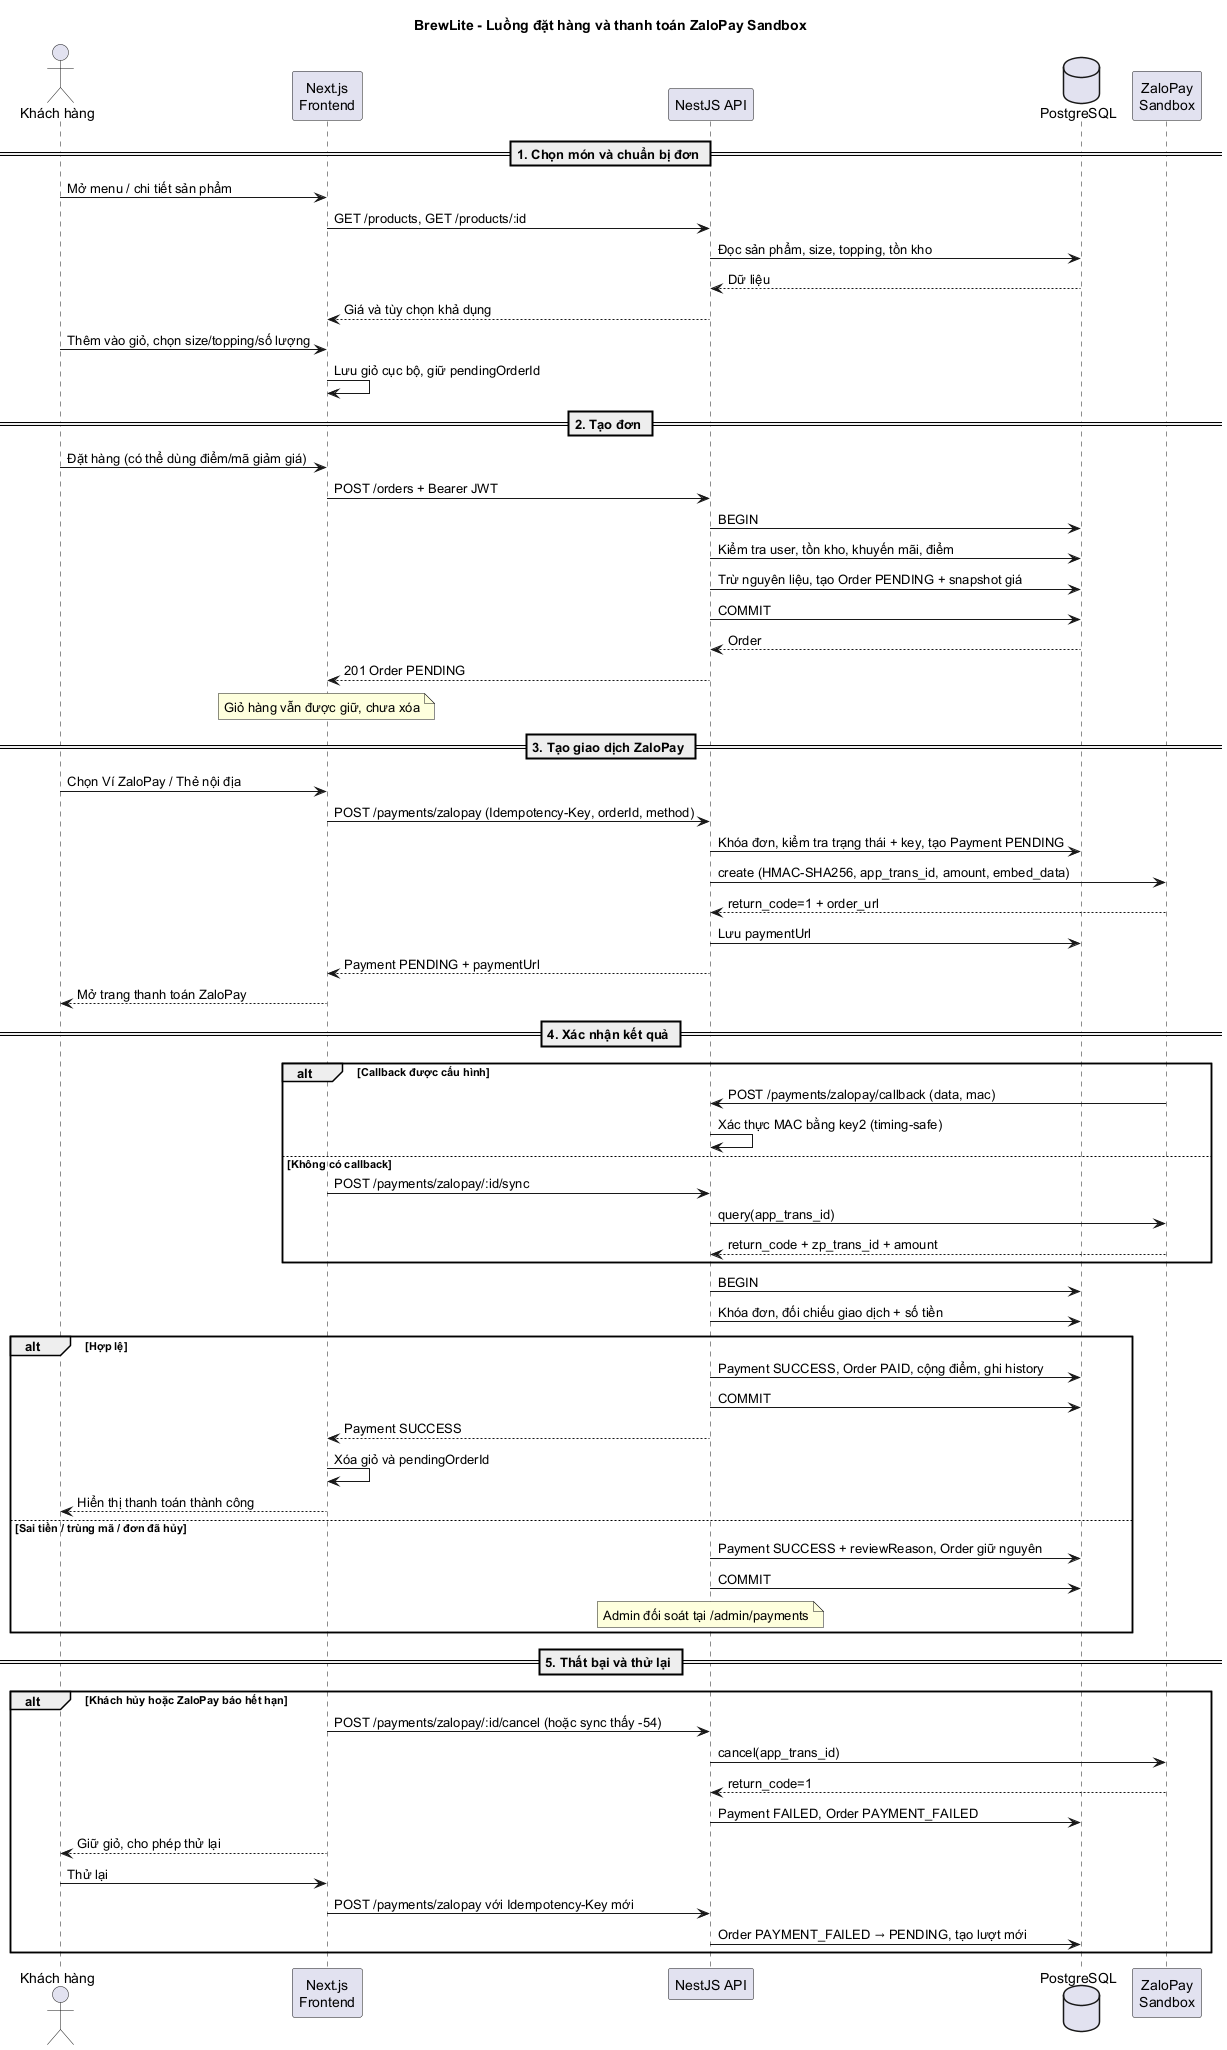
\includegraphics[width=0.95\textwidth]{../figures/diagrams/BrewLite-Checkout.png}
\caption{Sequence diagram luồng đặt và thanh toán đơn}
\label{figA:sequence}
\end{figure}

\paragraph{Giải thích các pha.}
% TODO(A): 4 đoạn ngắn: (1) xác thực + validate; (2) transaction tạo đơn + khoá tồn kho;
% (3) gọi ZaloPay + Idempotency-Key/request hash; (4) nhánh alt + callback/sync.
% Viết dạng đoạn văn hoặc danh sách sau khi soạn nội dung.

\subsection{Task 2.3 -- Class diagram}

% TODO(A): vẽ từ link draw.io, tối thiểu 7 lớp:
% User, Product, Order, OrderItem, Payment, Promotion, LoyaltyTransaction.
% Yêu cầu: thuộc tính chính, quan hệ, multiplicity, enum trạng thái.
% Nguồn dữ liệu: docs/database-design.md + apps/api/prisma/schema.prisma.
% Khi có file, đặt vào docs/diagrams/class-domain.svg (kèm nguồn draw.io/.puml)
% rồi bỏ comment khối hình dưới.
%
% \begin{figure}[H]
% \centering
% 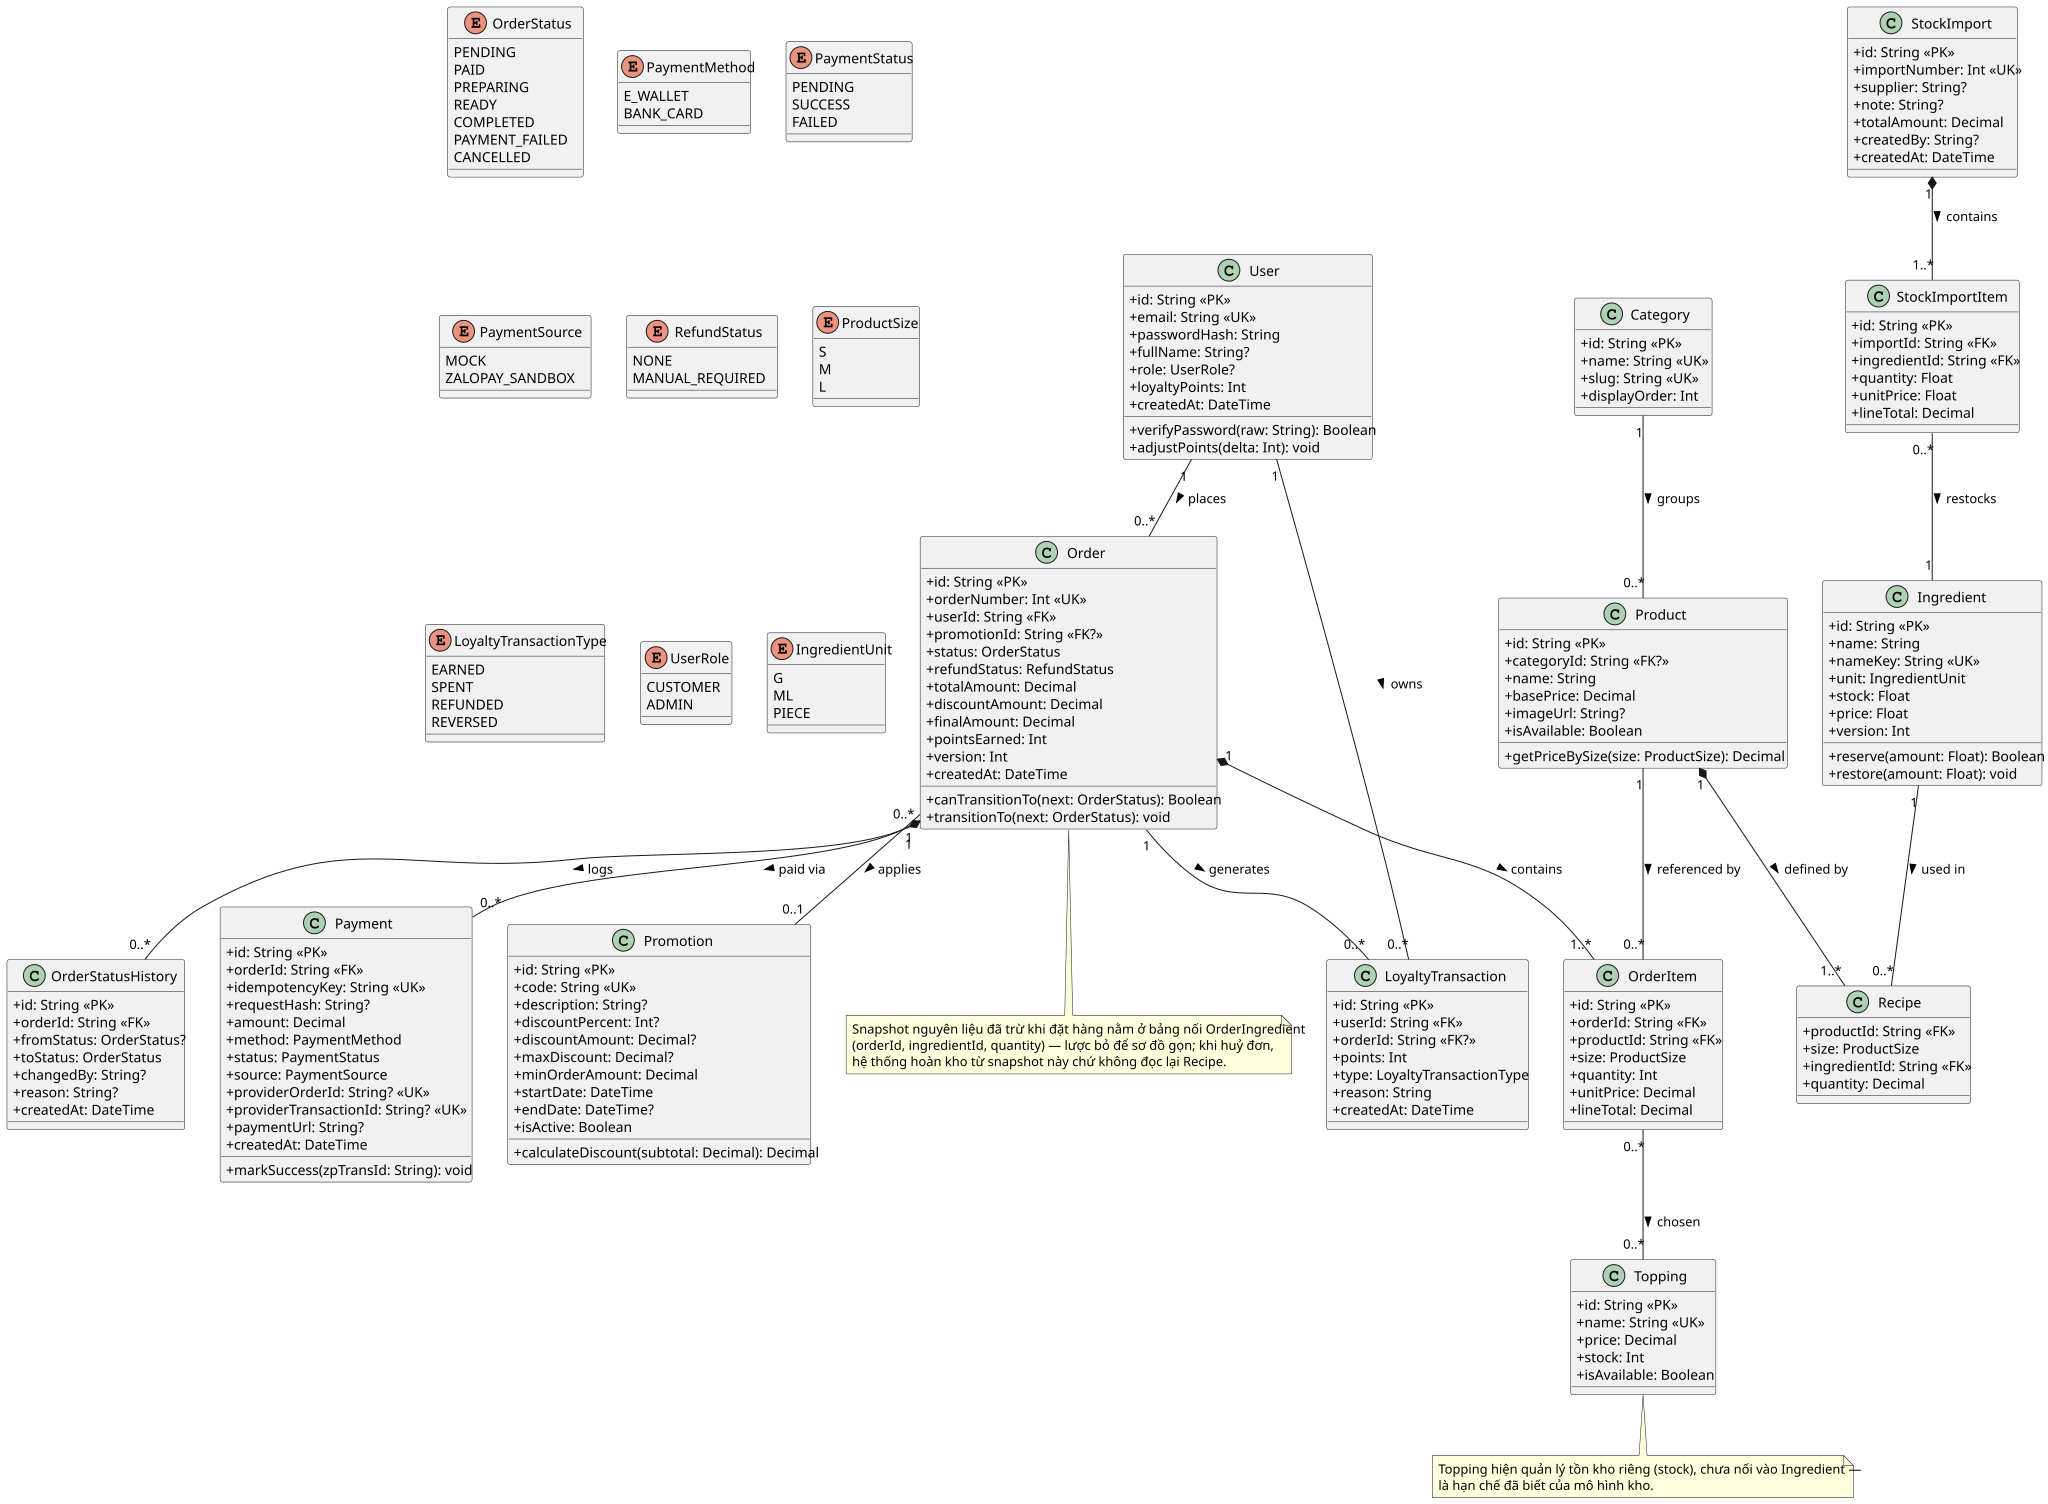
\includegraphics[width=0.95\textwidth]{../diagrams/class-domain.svg}
% \caption{Class diagram miền nghiệp vụ BrewLite}
% \label{figA:class}
% \end{figure}

\paragraph{Enum trạng thái.}
% TODO(A): bảng enum: OrderStatus (7 giá trị), PaymentStatus, RefundStatus, UserRole.
% Nguồn: docs/order/state-machine.md.
\begin{table}[H]
\centering\small
\caption{Enum trạng thái chính}
\label{tabA:enum}
\begin{tabularx}{\textwidth}{@{}l l X@{}}
\toprule
\textbf{Enum} & \textbf{Giá trị} & \textbf{Ý nghĩa} \\
\midrule
% TODO(A)
\bottomrule
\end{tabularx}
\end{table}

\subsection{Tính nhất quán giữa các mô hình}
% TODO(A): bảng đối chiếu -- tiêu chí nghiệm thu Task 2: 3 sơ đồ không mâu thuẫn SRS/use-case.
% Mỗi dòng: khái niệm | SRS | UC-01 | Activity | Sequence | Class
\begin{table}[H]
\centering\footnotesize
\caption{Đối chiếu khái niệm giữa SRS, use-case và ba sơ đồ}
\label{tabA:consistency}
\begin{tabularx}{\textwidth}{@{}l c c c c X@{}}
\toprule
\textbf{Khái niệm} & \textbf{SRS} & \textbf{UC-01} & \textbf{Activity} & \textbf{Sequence} & \textbf{Class} \\
\midrule
% TODO(A): ví dụ các dòng: Đơn PENDING, Trừ tồn kho, Idempotency-Key, Hoàn kho khi huỷ
\bottomrule
\end{tabularx}
\end{table}
